\chapter{Introducci\'o}

%primera versio d'estructura del document
\section{Entorn i eines de treball}
Totes les mesures, execucions i optimitzacions d'aquesta pràctica s'han dut a terme sota una arquitectura Intel Core Duo. Això ens permet treballar tant a les aules com en els nostres respectius portàtils.\\

Pel manteniment del codi i per poder treballar amb més facilitat hem optat per GIT com a sistema de control de versions. Concretament, hem optat per GitHUB \url{https://github.com/} que ofereix repositoris propis gratuïtament.

Per la feina propiament dita d'optimitzacions, hem utilitzat les eines vistes durant el curs. En el cas de fer servir alguna altra eina, ho indiquem en el document.

%scripts, makefile, etc
\section{Optimitzacions amb el compilador}
Al treballar sota una arquitectura Intel, tenim l'opció de treballar amb dos compiladors:

\begin{itemize}
  \item icc (ICC) 12.0.2 20110112
  \item gcc (Ubuntu/Linaro 4.5.2-8ubuntu4) 4.5.2
\end{itemize}

Sense començar a mirar el codi i per experiència d'anteriors pràctiques/feines, treballant sota una arquitectura Intel, el seu compil·lador natiu te millor rendiment. Tot seguit, adjuntem un benchmarking del codi, comparant els dos compil·ladors i emprant diferents flags. Pels flags del compil·lador d'Intel, hem seguit parcialment el manual d'optimitzacions d'Intel.

\begin{table}
\begin{center}
\begin{tabular}{lll}
\hline
 & ICC & GCC \\
\hline
\texttt{-O0} & 133.113s & 125.026s \\
\texttt{-O2} & 22.088s & 43.451s \\
\texttt{-O3} & 22.868s & 43.160s \\
\texttt{-O3 -march=core2} & 22.437s & 42.553s \\
\texttt{-O3 -parallel} & 33.690s & N.A.\\
\hline
\end{tabular}
\caption{Benchmarking entre compiladors i flags utilitzant el video del tigre}
\end{center}
\label{table1}
\end{table}

De seguida veiem que el codi te un rendiment molt superior tan aviat com se li apliquen optimitzacions. Això és una bo per nosaltres, ja que aplicant les millores vistes durant el curs directament sobre el codi, hauriem de tenir speedups que demostressin l'eficàcia d'aquestes optimitzacions.
Veiem també el que comentavem anteriorment, que sota una arquitectura Intel, el seu compilador és molt més eficient. Podriem dir que la versió \texttt{-O3 -march=core2} marca el millor temps que podem obtenir. Sembla dificil aconseguir millors optimitzacions que les més agressives que utilitza aquest compilador.
I finalment, com a curiositat, el flag \texttt{-parallel}, que intenta paralelitzar automaticament el codi, i en aquest cas correr sobre dos processadors, no aporta cap guany, al contrari, te un rendiment inferior.

%-O3, -march=core2 ... etc
\section{Profiling del codi original}

El primer pas abans de començar a treballar ha estat el de fer profiling del codi original, per tal d'identificar quines son les rutines que més temps de CPU consumeixen. Aix+o s'ha fet mitjançant l'eina \texttt{gprof} i posteriorment, dibuixant un graf que mostra visualment la sortida. De seguida veiem que la funció que més temps consumeix és \texttt{dist1} que alhora prové de la branca \texttt{motion}. Aquesta funció la trobem dins de \texttt{motion.c} i és la primera que optimitzarem.

\begin{figure}[hbtp]
\begin{center}
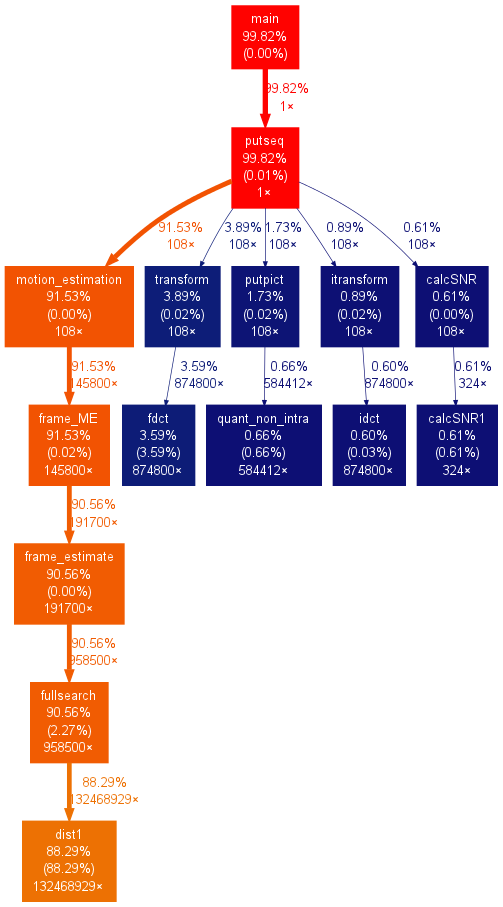
\includegraphics[scale=0.3]{img/output.png}
\caption{Graf del profiling del codi original}
\end{center}
\end{figure}

\section{Metodologia de treball}
Durant tota aquesta pràctica hem seguit la següent metodologia per validar i integrar les optimitzacions:

\begin{itemize}
  \item Codificar
  \item Testejar amb el fitxer tiger.mpg
  \item Comparar el resultat amb l'original (\texttt{diff})
  \item Calcular speedups
\end{itemize}
